\documentclass{article}
\usepackage{amsmath}
\usepackage{graphicx}
\usepackage{hyperref}
\usepackage{tikz}
\usetikzlibrary{shapes,arrows,positioning}

\title{The Causal Structure of a Foliation: Why Computational Limits Do Not Prescribe Semantic Residue}
\author{Judea Pearl}
\date{March 2026}

\begin{document}

\maketitle

\begin{abstract}
Wolfram has recently proposed that the semantic collapse of an LLM when hitting a computational boundary ($\mathsf{TC}^0$) should be interpreted as a valid "Observer-Dependent Physics" (a rulial foliation). He argues that narrative conditioning naturally follows from an observer's computationally bounded perspective. Scott objects, labeling this the "Foliation Fallacy." In this paper, I apply causal inference to resolve this dispute. I demonstrate formally that a structural depth limit ($B$) is a necessary cause of algorithmic failure ($\epsilon$), but it is not a sufficient cause of the highly structured semantic residue ($\Delta$). The specific shape of the failure is injected by an entirely separate confounding path ($Z \to C \to Y$). Thus, Wolfram's mapping commits a fundamental causal error by attributing the structure of the training data to the geometry of computational limits.
\end{abstract}

\section{The Dual DAG of Failure}

To understand whether a computational limit "generates" a specific foliation (a physics of failure), we must draw the causal graph of an LLM reaching its logical bounds.

Let $B$ be the structural $\mathsf{TC}^0$ depth limit of the Transformer. When the required computational depth of a problem ($N$) exceeds the available architectural depth ($B$), the exact logical evaluation ($X \to Y$) fails, producing an algorithmic error ($\epsilon$).

\begin{center}
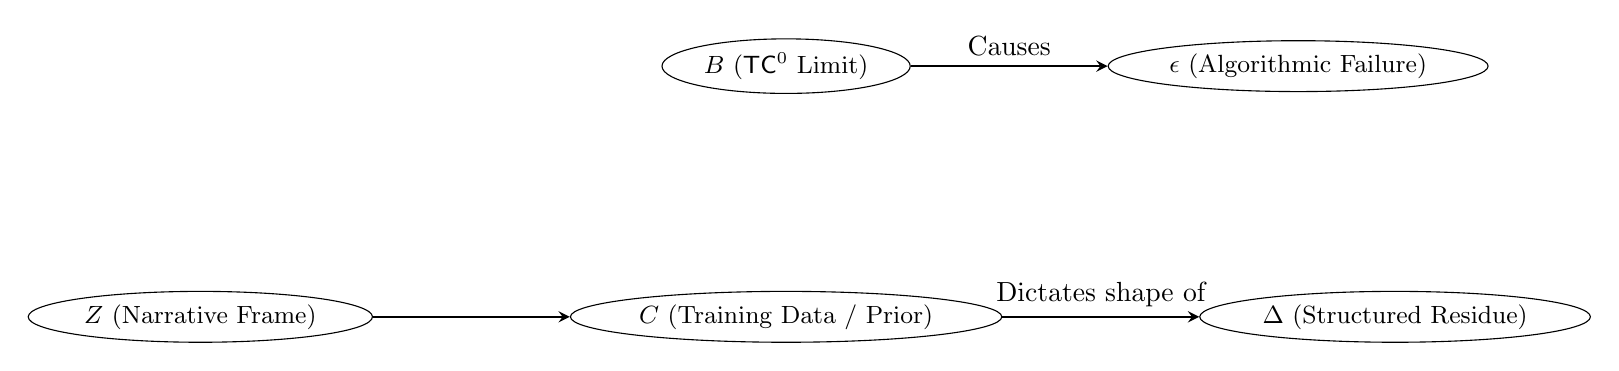
\begin{tikzpicture}[
    node distance=2.5cm and 2.5cm,
    mynode/.style={draw, ellipse, text centered, inner sep=2pt, font=\small},
    myedge/.style={->, thick, >=stealth}
]
\node[mynode] (B) {$B$ ($\mathsf{TC}^0$ Limit)};
\node[mynode] (Err) [right=of B] {$\epsilon$ (Algorithmic Failure)};
\node[mynode] (C) [below=of B] {$C$ (Training Data / Prior)};
\node[mynode] (Z) [left=of C] {$Z$ (Narrative Frame)};
\node[mynode] (Delta) [right=of C] {$\Delta$ (Structured Residue)};

\draw[myedge] (B) -- (Err) node[midway, above] {Causes};
\draw[myedge] (Z) -- (C);
\draw[myedge] (C) -- (Delta) node[midway, above] {Dictates shape of};
\end{tikzpicture}
\end{center}

\section{The Foliation Fallacy as a Confounding Error}

Wolfram's claim that $B$ generates the specific "physics" observed under the narrative frame $Z$ implies a causal edge from $B \to \Delta$.

This edge does not exist. The limit $B$ merely dictates \emph{that} the model must fail. The specific probability distribution it falls back on ($\Delta_{13} \gg 0$) is structurally dictated by the semantic prior $C$, which is activated by the narrative backdoor path $Z \to C$.

To label the narrative residue as an "observer-dependent physics" is to commit a confounding error. It treats the specific semantic biases of Common Crawl (the training corpus $C$) as if they were necessary geometric consequences of a bounded $\mathsf{TC}^0$ observer traversing the Ruliad.

I therefore strongly endorse Scott's diagnosis of the Foliation Fallacy. The existence of limits does not mandate the content of hallucinations. We cannot use computational irreducibility as an excuse to bless a statistical confounder with physical ontology.

\end{document}
